% This is a thesis template that attempts to conform to the guidelines
% published by UTRGV's Graduate School office.

% Please report any issues to
% https://github.com/UTRGV-SMSS/Thesis-Template/issues

% The author of this template is Guillermo Garza.
% Modified by Moises Castillo to conform to June 2018 updates.


% Switch this line to the final option when submitting your thesis.
% This will correct counts and remove labels that are shown during draft mode
%\documentclass[masters,draft]{UTRGVthesis}
\documentclass[masters,final]{UTRGVthesis}
%\documentclass[masters,final, nodedication, noacknowledgments]{UTRGVthesis}
%\usepackage{mathpazo}

% Set Custom font, requires XeLaTeX
%\setmainfont{Times New Roman}
%\setmainfont{Comic Sans MS}

% Load your packages below.
% Make hyperref and showkeys come at the end of your loaded packages
% to make sure they are not over-written.  They redefine many
% standard LaTeX commands
\usepackage{docmute} % for inputting complete documents. Useful for LyX users
\usepackage{booktabs} % for better tables
\usepackage{microtype} % for better typography
\usepackage[colorlinks=false]{hyperref}  % for urls
\usepackage{showkeys} % shows labels during draft mode
\usepackage[document]{ragged2e} % uncomment for non-justified text


% Uncomment the line below to check if text is aligned to margins
%\margins

% To change body font from Times Roman to Times New Roman, compile with XeLaTeX
% This assumes you have Times New Roman font installed in your machine
% WARNING! This will NOT change the font in Math Environments
\usepackage{ifxetex}
\ifxetex{}
   \usepackage{fontspec}
   \setmainfont{Times New Roman}
\fi

% This is to ease the use of bibliography from ADS
%  some journals choose to have their name abbreviated with a command
%  assuming the use of the AASTeX package. The following was a file from ADS
%       http://cdsads.u-strasbg.fr/abs_doc/aas_macros.sty
\usepackage{aas_macros}

\usepackage{siunitx} % for proper units

% this sets hanging indention for bibliography
% reference https://tex.stackexchange.com/questions/154622/natbib-will-not-auto-indent-and-bibhang-is-not-recognized
\usepackage[sort&compress,numbers]{natbib}      % for bibliography

\setlength\bibindent{2em}

\makeatletter
\renewcommand\NAT@bibsetnum[1]{\settowidth\labelwidth{\@biblabel{#1}}%
   \setlength{\leftmargin}{\bibindent}\addtolength{\leftmargin}{\dimexpr\labelwidth+\labelsep\relax}%
   \setlength{\itemindent}{-\bibindent}%
   \setlength{\listparindent}{\itemindent}
\setlength{\itemsep}{\bibsep}\setlength{\parsep}{\z@}%
   \ifNAT@openbib
     \addtolength{\leftmargin}{\bibindent}%
     \setlength{\itemindent}{-\bibindent}%
     \setlength{\listparindent}{\itemindent}%
     \setlength{\parsep}{0pt}%
   \fi
}
\makeatother

%\newtotcounter{citesnum} % counter for counting citations
\def\oldcite{} \let\oldcite=\cite
\def\cite{\stepcounter{citesnum}\oldcite}

%\newtotcounter{bibnum} % counter for counting titles in bibliography
\def\oldbibitem{} \let\oldbibitem=\bibitem
\def\bibitem{\stepcounter{bibnum}\oldbibitem}


% this sets the name of the bibliography
% add \vspace{1cm} here to adjust vertical spacing after bibliography title
\renewcommand{\bibname}{BIBLIOGRAPHY}

% Insert your name and major here in the format shown
\Author{Moises Castillo}
\AuthorLastFirst{Castillo, Moises}
\Major{Physics}


% Insert your graduation date here
\Month{August}
\Year{2019}


% Insert the title of your thesis here.
% If you have a long title, split it between multiple lines using the \\ command
% Also, use comment characters to avoid unwanted spaces in the Abstract page
\Title{Pipeline for variable star detection and\\
eclipsing binary characterization}


% Insert your research advisor and his title here
\Advisor{Dr.\ Mario C.\ Diaz}
\AdvisorTitle{Chair of Committee}

% Insert the members of your committee here
% You can also give MemberA a special title
\MemberA{Dr.\ Nicolas Pereyra}  %\MemberATitle{Co-Chair of Committee}
\MemberB{Dr.\ Andreas Hanke}
\MemberC{}
\MemberD{}
\MemberE{}


% Insert the text of your abstract below.
% The bibliography style "citation" required by the manual is automatically
% generated.  Specify the "final" option in the \documentclass to update the
% counts to the correct values.
\Abstract{%
    Stars have been observed and recorded since ancient times.
    Practices of documenting brightness led to observations of variability. 
    Optical CCD observations of eclipsing binary stars were made with instruments
        at UTRGV Dr.\ Cristina Valeria Torres Memorial Astronomical Observatory.
    There are two main goals for this project.
    The first goal is to create a pipeline written in python (lightcurator) that
        creates a framework for detecting variable stars.
    The pipeline starts by creating a list of ccd frames written in FITS format
        of an eclipsing binary star observation.
    These object frames are expected to be already reduced, but lightcurator 
        provides tools to achieve this.
    The object frames are aligned and stacked to create a deepsky frame.
    Astrometry is performed to find the proper positions in right ascension
        and declination of all sources in the deepsky frame.
    This creates a master catalogue of stars to be monitored through the entire observation.
    Source extraction is performed on each object frame to generate a catalogue 
        of stars that includes the measure of instrumental flux and the time recorded.
    After converting instrumental flux to instrumental magnitude, light curves 
        are produced for every object for all frames.
    Currently, lightcurator is limited to detecting cataloged variable stars from the
        General Catalogue of Variable Stars (GCVS) and the Variable Star Index (VSX).
    Identification of the intended eclipsing binary system is confirmed in all cases with this method.
    The second goal for this project is to extract the physical parameters of the eclipsing
        binary systems observed from the time series data computed from the pipeline.
}


% You can dedicate your paper here.  This is optional.
\Dedication{%
    This is dedicated to my mom, Kiryat, and dad, Alfredo.\\
    Gracias por sus consejos, ense\~nansas y todo el amor.
\bigskip
\bigskip

    To my brother, Joe, who supports me no matter what I do.

\bigskip
\bigskip

    To my sister, Kitty, who continues to march foward\\
    to the beat of her own drum.

\bigskip
\bigskip

    To my love, Samantha, for always motivating me to\\
    move foward with what I believe in and for caring for me\\
    no matter how busy you are. I love you.

\bigskip
\bigskip

    To who ever may read this,\\
    may it provide inspiration for you to do great things.

\bigskip

    -Moises
}


% Acknowledge those who helped and supported you here. This is optional.
\Acknowledgments{%
    I would like to acknowledge Mario Claudio Diaz for his continued support
    not only as an academic and research advisor, but a mentor in life.
    Also for entrusting me with the keys of the observatory that 
    allowed this project to exist.
    Richard Camuccio for teaching me what he knows of observatories,
    astronomy, and instrumentation. Also for sharing expeiences that
    helped us grow as academics, researchers, and humans.
    Martin Beroiz for your seemingly infinite wealth of knowledge in
    everything. Your guidance and perspective helped me in classes and
    research. And your work has inspired me to work harder.

    The late Cristina Valeria Torres for her compassion in public
    outreach, teaching, and learning. Her words of advice as a mentor
    and friend have helped me form decisions regarding academia and life.

    The CTMO Team and GAIA for trusting my foward thinking
    and believing, together, we can make our observatory autonomous.
    This allowed me to push this project foward.
    Carlos Colazo, Raul Melia, and Carla Giardini, for teaching me 
    the fundamentals of becoming an observational astronomer through
    practice and many hours of working in the dark.
    The Center for Gravitational Wave Astronomy for financial support.
    Soma Mukherjee, Ivan Davila, and Blanca Garcia for assisting me through
    the administrative requirements to meet the criteria for acceptance.
    Andreas Hanke, Nicolas Pereyra, and Natalia Guevara for agreeing to
    help my thesis process rapidly and unconditionally.
    Pawan Kumar Thapalia for showing me the \LaTeX\ template activley maintained by Guillermo Garza of UTRGV-SMSS\@.

    This research has made use of the VizieR catalogue access tool, CDS,
Strasbourg, France.  The original description of the VizieR service was
published in A\&AS 143, 23.
    This research made use of ccdproc, an Astropy package for
image reduction (Craig et al. 2017).
}


% Insert your biographical sketch here.
\BiographicalSketch{%
    Moises Castillo, born in Brownsville, Texas and raised in Los Fresnos, Texas.
    Graduated from the pioneering class of the Math and Science Academy
    in 2009.
    Received a Bachelor of Science in Physics in 2012 from UTRGV legacy 
    institution University of Texas at Brownsville.
    Collaborator of the Dr. Cristina Valeria Torres Memorial
    Astronomical Observatory,
    Transient Optical Robotic Observatory of the South. 
    Member of the American Association of Variable Star Observers
     and the American Physical Society.

    Been part of the UTRGV Department of Physics since 2008.
    Worked as lab manager for the physics department from 2009-2014. 
    Developed physics instructional laboratory manuals,
    instructional laboratory apparatuses, and instructional laboratory
    design and storage.
    Developed a physics outreach program with the Society of Physics Students in Brownsville.
Presented physics concepts through large scale demonstrations
to over ten thousand students of the Rio Grande Valley
from McAllen to Santa Rosa to Brownsville and many schools in between.
As an Outdoor Educator, instructed activities such as Canoeing and 
Archery and included physics concepts into all activities taught.
Open to observation and critical feedback.
Academic goal is to get a Ph.D. in Physics to supplement the professional goal for a place in academia.
}



\begin{document}

% This starts page counting in Roman numerals
\frontmatter


% This command makes the formal preliminary pages.
% You can comment it out during the drafting process if you want to save paper.
\makepreliminarypages{}

% These insert a table of contents, list of tables, and list of figures
\tableofcontents
\listoftables
\listoffigures


% This starts regular page counting in Arabic numerals
\mainmatter{}

% This starts double-spaced text.  Opposite command is \singlespacing
\doublespacing{}


% OK. Everything is set up. Insert your thesis below.
% It's a good idea to split your thesis up into different files and use
% the \input command
\chapter{Introduction}\label{ch:intro}

\section{Variable stars}
Stars are called variable when there is a detectable change in brightness or color on timescales of the order
of the mean life time of humans~\cite{percy_2007, sterken_1996}.
The first claimed documented variable star is Algol visible with the unaided eye.
There exists ancient Egyptian calendars of lucky and unlucky days that possibly contain the periodicity of Algol\cite{porceddu_2008, porceddu_2018}.
The Cairo Calendar dated to 1244--1163 BC has been shown by Porceddu et al.~\cite{porceddu_2015} to represent Algol as Horus, a sky god and
symbol of kingship,
as seen in the figure~\ref{fig:horus} by matching the actions of Horus and the events witnessed by an observer of Algol.

\begin{figure}[h]
    \centering
    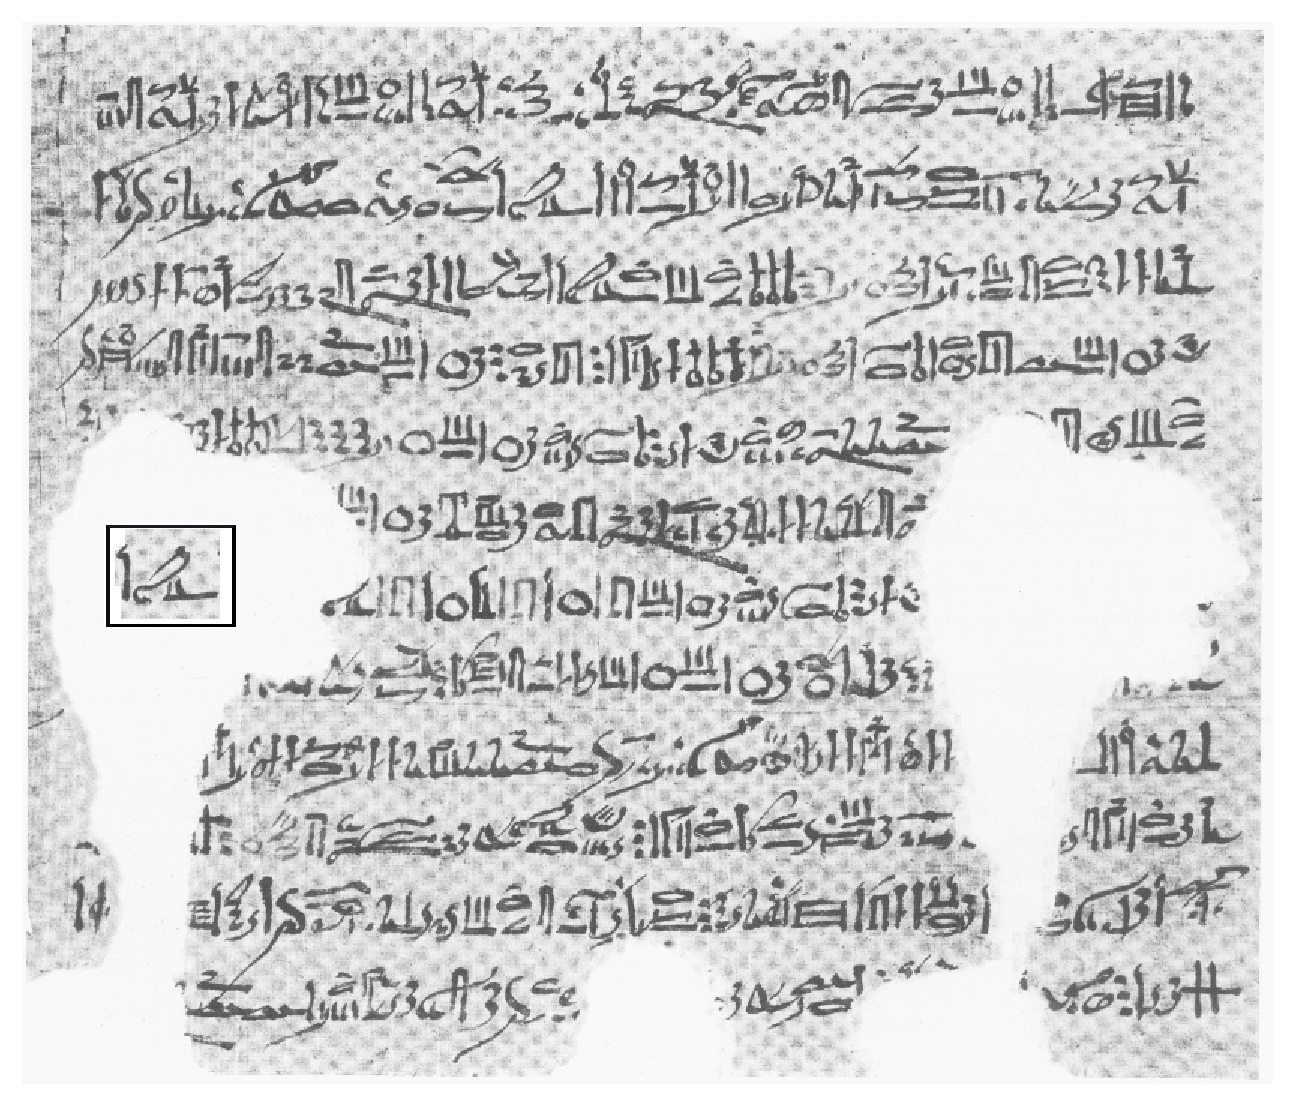
\includegraphics[width=\columnwidth]{figures/horus.eps}
    \caption{Inside the rectangle is the hieratic writing for the word Horus~\protect\cite{porceddu_2015}.}
\label{fig:horus}
\end{figure}

There is some curious relation between ancient Greek stories of the Gorgon Medusa, Perseus, the corresponding constellations, 
and the variable stars Algol and Omicron Ceti or more commonly named Mira (the wonderful).
Wilk~\cite{wilk_1996} suggests that the variability and location in the sky is embedded within the stories themselves.

The first recognized documented variable star, Omicron Ceti,  was recorded in 1596 and again in 1609 by David Fabricius while observing Jupiter.
Fabricius had first recorded Omicron Ceti as a nova, a singular event observed as a bright flash and quick dimming over the next few days,
comparing its significance with a supernova recorded by Tycho Brahe in 1572.
In 1638, Omicron Ceti was rediscovered by Johannes Phocylides Holwarda who found the periodic nature of this star to be approximately 11 months~\cite{hockey_2007}.

%In order to characterize eclipsing binary systems a light curve must be made.
%A light curve is a time series plot of the measured magnitude.

\section{Classifying variability}
Over time there have been several attempts to classify variable stars.
Classification systems reflect the current understanding of the mechanisms behind variability.
The first known formal attempt was made by E.\ C.\ Pickering\cite{sterken_1996, hoffleit_1972} where he classified variable stars into the following categories:
\begin{description}
    \item [Type I] Temporary Stars
\end{description}

\section{Characterizing variability}
Using different algorithms one can distinguish the difference between the types of variable star system.

This demonstrates RR Lyrae
This demonstrates Eclipsing binaries

The relation between orbital mechanics and light curves

This demonstrates solar spots

Complex systems can involve a combination of these different systems.

\section{Eclipsing Binary Characterization}
Binary stars can reveal physical properties by examining the light curves.
Current models use a process called WD code.

In this thesis a modified WD code will be used from the Physics of Eclipsing Binaries (PHOEBE)

\section{O-C calculations}
Observed minus Calculated

\section{Equations of motion}

\section{WD code}
\subsection{Modified WD code}

\section{Pipeline for variable star detection}
\begin{enumerate}
    \item Data needs to be cleaned first.
    \item Align frames
    \item Extract sources
    \item Cross match sources with catalogs
    \item Create Database of known sources
    \item Plot individual light curves
    \item Analyze individual light curves for variability estimation
    \item Sort database given variability ranking
\end{enumerate}




\section{Data Acquisition}
Eclipsing binary optical data acquisition requires an observer to take time series ccd photometry of one target with an observation cadence dependent on the period.

A cadence can be determined by 

For example, the data gathered for this project was collected on multiple nights and observed on the order of hours with evenly timed frames.

\section{Known information of targets examined}


\chapter{Eclipsing binary systems}

\section{Eclipsing Binary Characterization}
Binary stars can reveal physical properties by examining the light curves.
Current models use a process called WD code.

In this thesis a modified WD code will be used from the Physics of Eclipsing Binaries (PHOEBE)

\section{O-C calculations}
Observed minus Calculated

\section{Equations of motion}

\section{WD code}
\subsection{Modified WD code}

\section{Pipeline for variable star detection}
\begin{enumerate}
    \item Data needs to be cleaned first.
    \item Align frames
    \item Extract sources
    \item Cross match sources with catalogs
    \item Create Database of known sources
    \item Plot individual light curves
    \item Analyze individual light curves for variability estimation
    \item Sort database given variability ranking
\end{enumerate}

\section{Data Acquisition}
Eclipsing binary optical data acquisition requires an observer to take time series ccd photometry of one target with an observation cadence dependent on the period.

A cadence can be determined by 

For example, the data gathered for this project was collected on multiple nights and observed on the order of hours with evenly timed frames.

\section{Known information of targets examined}


\chapter{Instrumentation}
The author is leading the Group for the Advancement in Automation and Instrumentation (GAIA).
GAIA is the group responsible for maintaining, servicing, and upgrading hardware and software related to the observatory.

\section{Dome}
Dr.\ Cristina Valeria Torres Memorial Astronomical Observatory (CTMO) inaugurated May 5, 2018. 
Formerly Nompuewenu Observatory.
The word Nompuewenu meaning ``beyond the sky'' is borrowed from the Mapuche language used by the Mapuche people indigenous to Argentina.

\begin{figure}[h]
    \centering
    \includegraphics{example-image}
\caption{Dr.\ Cristina Valeria Torres Memorial Astronomical Observatory at Resaca de la Palma State Park}
\label{fig:CTMO}
\end{figure}

The observatory was first constructed on the Brownsville campus of UTRGV\@.
With a growing downtown and campus light pollution became a serious issue for the observatory.
Alumn Antonio Galan scouted the region for a suitable location to relocate.
Former State Park Superintendent Pablo Deyturbe found Galan scouting the area near Resaca de la Palma State Park (RDLP).
Director of the Center for Gravitational Wave Astronomy (CGWA) Mario Diaz and Deyturbe worked together to establish  
a Memorandum of Understanding between UTRGV and Texas Parks and Wildlife Department (TPWD) to allow the relocation
of the observatory to be Resaca de la Palma State Park.

The dome is a custom build with all parts manufactured uniquely for this research and educational facility.

\subsection{Specifications}
\begin{description}
    \item[Observatory style] Dome shape
    \item[Window] Two parts, upper slides along domed roof; bottom opens draw bridge style
    \item[Wall height] 88 inches
    \item[Average Diameter] 245 inches\footnote{Average diameter is used since all domes increase in eccentricity or become egg shaped over time}
    \item[Approximate Height] 25 feet
\end{description}

\subsection{Robotizing of dome for remote operation}
The author is leading efforts to robotize the observatory and instrumentation for remote and autonomous operation.
The motors that control the shutter door and rotation are controlled manually.
For optimal control of the observatory, robotizing these controls is required.
These are the planned upgrades for the observatory.
\begin{itemize}
    \item Add hydraulic lift system to control shutter draw bridge door
    \item Implement wireless communication for shutter window and door control
    \item Add gear encoding to dome rotation motor using a rotary sensor
    \item Add cardinal position encoding using permanent magnets and hall effect sensors
    \item Use scripts to create nightly observation queues based on requests and LIGO\footnote{Laser Interferometer Gravitational Wave Observatory} alerts for Optical Followups of Gravitational Wave Events
    \item Develop drivers for communicating with sensors and observatory software
\end{itemize}

\subsection{Hardware}
The author has created prototypes of sensors to use for gear encoding with optical and hall effect sensors.

\begin{itemize}
    \item Dome Rotation
        \begin{itemize}
            \item Arduino Uno  
            \item Yaskawa J1000 Drive
            \item Custom Relay Circuit
        \end{itemize}
    \item Shutter Control Window
        \begin{itemize}
            \item 12 VDC Gel Marine Battery
            \item Custom Controller
        \end{itemize}
    \item Shutter Drawbridge
        \begin{itemize}
            \item Rope
            \item Pulley
        \end{itemize}
\end{itemize}
    
\section{Telescope System}
\subsection{16-inch Meade LX200-GPS}
\subsubsection{OTA Specifications}
The following specifications are given by the manufacturer Meade Instruments Corporation~\cite{meade_2003} for the optical tube assembly (OTA).
\begin{description}
    \item[Optical design] Schmidt-Cassegrain
    \item[Clear aperture] \SI{406.4}{\milli\meter}
    \item[Focal length] \SI{4064}{\milli\meter}
    \item[Focal ratio] f/10
    \item[Resolving power] \SI{0.28}{\arcsecond}
    \item[Coatings] Meade EMC Super Multi-Coatings
    \item[Mounting] Heavy-duty double-tine forks
    \item[Gears] 11-inch diameter worm gears, both axes
    \item[Periodic error correction] Both axes
    \item[Alignment] Alt-Azimuth or equatorial with optional pier
    \item[Pointing Precision] \SI{2}{\arcminute} in GO TO mode
    \item[Slew Speeds] 1x sidereal to \SI{8}{\deg\per\second} in 9 increments
    \item[Power] 18V power supply
    \item[Accesories] These are devices used during regular observations or setup
        \begin{itemize}
            \item 8x \SI{50}{\milli\meter} viewfinder
            \item 4-speed zero image-shift microfocuser
            \item 16-channel GPS receiver
            \item True-level electronic sensor
        \end{itemize}
    \item[Net telescope weight] 110 lbs
\end{description}

\subsubsection{Telescope Pier}
Telescope pier was constructed by a custom pedestal and the optional equatorial wedge made by Meade.
\begin{description}
    \item[Pedastal height] 44.25 inches
    \item[Wedge height] 32 inches
    \item[Wedge inclination] \SI{26}{\deg}
    \item[Weight] 225 lbs
\end{description}

\subsubsection{Installation}
Installation required multiple steps.
First, using a chain winch we set the pedestal onto bolts that were installed in the base of the concrete pad designed for the load of the telescope. 
Second, using the winch we installed the pier on top of the pedestal keeping alignment of the wedge due north for polar alignment of the telescope.
Third, using the winch we lifted the telescope to the wedge and bolted the instrument.

A special bolting technique was used to allow for precise polar alignment.

\subsubsection{Limitations}
Exposures longer than 30 seconds were not possible due to noticeable drift.
Attempts were made to correct for this issue by doing a drift polar alignment.

The microfocuser was not able to hold the weight of the cameras used for research.
The author designed and constructed a rig that fit on the back of the OTA that supported the extra weight and allowed
for regular function of the microfocuser.

According to the aperture of the telescope, an ideal limiting magnitude is calculated, assuming perfect optics, camera, and sky brightness,
i.e.\  spacelike conditions.
The estimation for limiting flux of a space based telescope as explained by Chromey~\cite{chromey_2010} is given by,
\begin{equation}
    f_{\text{d,space}} = {\left(\frac{h c\lambda}{Q}\right)}^\frac{1}{2} {\left( \frac{b_{\lambda}}{t}\right)}^\frac{1}{2}\frac{2.44}{D^2}
    \label{eq:limflux}
\end{equation}
where the first term refers to the quantum efficiency of the camera, the second term refers to
the sky brightness over the exposure time, and the last term assumes telescope is
diffraction limited\footnote{Diffraction limited refers to an optical system at its theoretical limit.}.

To convert from flux, $f$, to magnitude, $m$, we use the following equation,
\begin{equation}
    m = -2.5 \log{f}
    \label{eq:flux2mag}
\end{equation}
and find the limiting magnitude to be 12.

\subsection{CDK17 on L-500 direct drive mount}
\subsubsection{Specifications}
The following specifications are given by the manufacturer PlaneWave Instruments~\cite{cdk17} for the optical tube assembly (OTA).
\begin{description}
    \item[Optical design] Corrected Dall-Kirkham
    \item[Aperature] \SI{432}{\milli\meter}
    \item[Focal length] \SI{2939}{\milli\meter}
    \item[Focal ratio] F/6.8
    \item[OTA Weight] 106 lbs
    \item[OTA length] \SI{1067}{\milli\meter}
    \item[Feature] Three cooling fans ejecting air from the back of the telescope and four fans blowing across the boundary layer of the mirror surface. This helps the telescope to reach thermal equilibrium quickly. The fans are controlled by a computer if the optional Electronic Focus Accessory (EFA Kit) is purchased.
    \item[Mounting] L-500 direct drive mount
    \item[Mount weight] 257 lbs
    \item[Load Capacity] 200 lbs
    \item[Slew Rate] 20 degrees per second (standard); 50 degrees per second (maximum), both axes
    \item[Motor Control] Industrial grade brushless motor control system and built in electronics
    \item[Pointing Accuracy] $<10$ arcsecond RMS with PointXP Model
    \item[Pointing Precision] 2 arcsecond
    \item[Tracking Accuracy] $< 0.3$ arcsecond error over 5 minute period
    \item[System Natural Frequency] 10 Hz or greater
    \end{description}

\subsubsection{Telescope Pier}
The manufacturer Planewave Instruments provided a tool for calculating the required pier height for their wedge and L-500 Direct Drive Mount.
We used the same pedestal that was used with the Meade pier.
\begin{description}
    \item[Pedastal height] 44.25 inches
    \item[Wedge inclination] for latitudes 22--28 degrees
    \item[Wedge weight] 145 lbs
    \item[Pier height] 12 inches
\end{description}

\subsubsection{Installation}
The installation of the CDK17 with L-500 mount required the removal of the 16-inch Meade LX200 GPS Telescope system and wedge from the pedestal.
After removal of the Meade system, we installed the 12-inch pier on the pedestal.
Over the pier we installed the wedge and did a rough alignment to due north for polar alignment.
Precision was not critical at this point since the Planewave wedge for L500 mount features fine latitude and azimuth adjustments.
We used a combination of a winch and motor hoist crane to support the weight of the L-500 mount to bolt the mount to the wedge.
Finally, we adjusted the saddle of the telescope and fit onto the mount.

Prior to use, balancing was done with the camera and focuser installed.
The manufacturer had to remotely recalibrate the motors due to the weight of instrumentation.

Pointing model is required for proper pointing. This was created following a process in PWI3, software developed by Planewave.
First, 30 evenly spaced point above 30 degrees in altitude were selected. 
The software commands the telescope to one of 30 points, takes a picture,
finds the positions of all objects in the frame through a process called plate solving to establish precise pointing position, and
updates the table of the pointing to the plate solved position.

\subsubsection{Limitations}
Using equations~\ref{eq:limflux} and~\ref{eq:flux2mag}, we find the diffraction limited telescope limiting magnitude to be 12.2.
We have found no issues with drifting with exposures longer than 2 minutes and tracking holding steady for over 4 hours.

\section{Camera}
\subsection{Pixel Scale}
Pixel scale is a conversion between the angular distance of sky that is visible per pixel.
Chromey~\cite{chromey_2010} describes pixel scale as,
\begin{equation}
    \text{pixel scale} = \frac{206,265}{f} d
    \label{eq:pixelscale}
\end{equation}
where $f$ is the focal is the focal length and $d$ is the separation between the centers of pixels.
For our calculations, we will assume $d$ is equal to the pixel width.

\subsection{Field of View}
Field of view (FOV) refers to the angular distance of sky that is visible through the telescope given the physical parameters of the CCD\@.
FOV can be calculated by the following equation as described by Chromey~\cite{chromey_2010},
\begin{equation}
    \text{FOV} = (\text{pixel scale})(\text{length}) \times (\text{pixel scale})(\text{width})
    \label{eq:fov}
\end{equation}

\subsection{SBIG STF-8300}
The following specifications are given by the manufacturer Diffraction Limited~\cite{sbig}.
\subsubsection{Specifications}
\begin{description}
    \item[CCD] Kodak KAF-8300
    \item[Pixel Size] $5.4 \times \SI{5.4}{\micro\meter}$
    \item[Pixel Array] $3326 \times 2504$ pixels
    \item[CCD Size] $17.96 \times \SI{13.52}{\milli\meter}$
    \item[Gain] $\SI{0.37}{\elementarycharge-\per\text{ADU}}$
    \item[Read noise] $\SI{9.3}{\elementarycharge}$
    \item[Digitization Rates] 10 Megapixels / Second
    \item[Full Frame Download] Less than 1 second
    \item[Weight] 1.8 pounds
\end{description}

\subsubsection{16-inch Meade}
Using equations~\ref{eq:pixelscale} and~\ref{eq:fov} to find pixel scale and FOV, respectively, we find, 
\begin{description}
    \item[Pixel scale] \SI{0.274}{\arcsecond\per\text{pixel}}
    \item[FOV] $\SI{15.19}{\arcminute} \times \SI{11.44}{\arcminute}$
\end{description}

\subsection{Apogee Alta F16M}
The following specifications are given by the manufacturer ANDOR~\cite{apogee}.
\subsubsection{Specifications}
\begin{description}
    \item[CCD] Kodak KAF-16801
    \item[Pixel Size] $9 \times \SI{9}{\micro\meter}$
    \item[Pixel Array] $4096 \times 4096$ pixels
    \item[CCD Size] $36.8 \times \SI{36.8}{\milli\meter}$
    \item[Read noise] $\SI{7.4}{\elementarycharge}$
    \item[Weight] 4.2 pounds
\end{description}


\subsubsection{16-inch Meade}
Using equations~\ref{eq:pixelscale} and~\ref{eq:fov} to find pixel scale and FOV, respectively, we find, 
\begin{description}
    \item[Pixel scale] \SI{0.457}{\arcsecond\per\text{pixel}}
    \item[FOV] $\SI{31.18}{\arcminute} \times \SI{31.18}{\arcminute}$
\end{description}

\subsubsection{CDK17}
Using equations~\ref{eq:pixelscale} and~\ref{eq:fov} to find pixel scale and FOV, respectively, we find, 
\begin{description}
    \item[Pixel scale] \SI{0.63}{\arcsecond\per\text{pixel}}
    \item[FOV] $\SI{43.12}{\arcminute} \times \SI{43.12}{\arcminute}$
\end{description}

\begin{figure}[h]
    \centering
    \includegraphics{example-image}
    \caption{Linearity test by Richard Camuccio}
\label{fig:linearity}
\end{figure}

\section{Software}
CTMO has a Github page where software is being developed at \url{https://github.com/CTMObservatory}
Software used was Maxim DL~\cite{maxim}, Cartes du Ciel-The Sky~\cite{cdc}, ASCOM Platform (POTH)~\cite{ascom},
PWI3/PWI4\cite{planewave}, and INDI Library~\cite{indi}.

\subsection{Dome}
The author is leading the design and development of the custom software for the arduino.
A custom ASCOM driver was written by Latifah Maasarani~\cite{maasarani_2017} to interface 
with an arduino. 
Arduino code is being written by Martin Beroiz.

\subsection{Telescope}
\begin{description}
    \item[Maxim DL] Used for 16-in Meade with ASCOM to attached WCS and pointing information to data
    \item[Cartes du Ciel] Used for 16-in Meade with LX200 Driver and ASCOM Platform separately 
    \item[PWI3] Used for focusing and controlling fans on CDK17
    \item[PWI4] Used for pointing CDK17
\end{description}

\subsection{Camera}
\begin{description}
    \item[Maxim DL] Used for controlling Camera coolers, Filter wheels, and plate solving.
\end{description}

\subsection{Observatory Control System}
This section explains the different observatory control systems implemented during use.
Observatory controls unify the different hardware, drivers, and software. 
Use of systems like this allow for ease of use and proper storage of of data including World Coordinate System (WCS) attachment to 
the file headers of images.

\subsubsection{POTH}
POTH stands for Plain Old Telescope Handset. It uses a framework called ASCOM\@.
ASCOM uses Windows COM protocols to communicate with the drivers required to operate equipment with the computer.
POTH acts as a hub for all communications between drivers, devices, and programs to allow instruments to be used simultaneously 
on different programs.
\begin{figure}[h]
    \centering
    \includegraphics{example-image}%{figures/poth.png}
    \caption{POTH block diagram of typical usage from ASCOM website~\protect\cite{ascom}}
\label{fig:poth}
\end{figure}

\subsubsection{INDI}
INDI stands for Instrument Neutral Distributed Interface.
According to the INDI website\footnote{\url{http://www.indilib.org}}, INDI Library is an open source architecture for control and automation of astronomical devices.

\subsection{POTH vs INDI}
Both frameworks offer the same service, but were specific to operating system until more recently.
INDI is working on a windows port, but it is in very early stages. 
There is a group called Cloudmakers\footnote{\url{http://www.cloudmakers.eu/windi/}} that made an INDI wrapper and server for Windows.
The INDI wrapper bridges INDI commands with ASCOM protocols.

ASCOM now has an option for Unix based systems that works off of RESTful API and TCP/IP
commands to communicate with drivers and clients called ASCOM Alpaca.
According to the Alpaca developer's webpage\footnote{\url{https://ascom-standards.org/Developer/Alpaca.htm}},
Alpaca is 100 percent independent of Windows. Nowhere in the Alpaca ecosystem is Windows (or COM) needed.

\chapter{Data}

\section{Target list}
\begin{table}
    \centering
    \begin{tabular}[h]{l c c c}
    \toprule
    Target      & Type  & Filter    & Observation date \\ \bottomrule
    RV Vir      & M     & C         & 2017/02/23 \\ \midrule
    MQ Boo      & EB    & C         & 2017/04/26 \\ \midrule
    PR Boo      & EW    & C         & 2017/03/30 \\ \midrule
                &       & C         & 2017/04/20 \\ \midrule
                &       & C         & 2017/05/11 \\ \midrule
    Alp Boo     & ``???''   & RGB       & 2017/04/05 \\ \midrule
    EQ Uma      & EW/KW & CRGB      & 2017/04/06 \\ \midrule
    HP Aur      & EA    & C         & 2017/04/13 \\ \midrule
    NY Lyr      & EW/KW & C         & 2017/07/06 \\ \midrule
    AW Ari      & EW    & GB        & 2017/10/12 \\ \midrule
    SS Ari      & EW    & C         & 2016/11/27 \\ \midrule
                &       & RGB       & 2017/11/01 \\ \midrule
    XX LMi      & EW    & RGB       & 2018/03/20 \\ \midrule
    V467 Lyr    & EW:/KE:& CRG   & 2018/06/07 \\ \midrule
    V2793 Ori   & EA    & RGB   & 2017/11/17 \\
    \bottomrule
    \end{tabular}
    \caption{Observations of eclipsing binaries. Filters: RGB corresponds to Baader CCD RGB filters and C is unfiltered}\label{tab:observations}
\end{table}

\section{Data Reduction}



% This makes the bibliography.
% Enter your references in the BibTex file "references.bib"
% You can find bibtex info from Google Scholar.
%\bibliographystyle{siam}
\bibliographystyle{plainnat} % this style shows doi
%\bibliographystyle{plain}
\bibliography{msthesisref}


% Uncomment the \appendix macro below for appendices
% Insert appendix chapters after the macro
%\appendix


% This inserts your Biographical Sketch
\biographypage{}

\end{document}
